%%%%%%%%%%%%%%%%%%%%%%%%%%%%%%%%%%%%%%%%%%%%%%%%%%%%%%%%%%%%%%%%%%%%%%%%%%%%%%%%%%%%%%%%%%%%%%%%
%
% CS484 Written Question Template
%
% Acknowledgements:
% The original code is written by Prof. James Tompkin (james_tompkin@brown.edu).
% The second version is revised by Prof. Min H. Kim (minhkim@kaist.ac.kr).
%
% This is a LaTeX document. LaTeX is a markup language for producing 
% documents. Your task is to fill out this document, then to compile 
% it into a PDF document. 
%
% 
% TO COMPILE:
% > pdflatex thisfile.tex
%
% If you do not have LaTeX and need a LaTeX distribution:
% - Personal laptops (all common OS): www.latex-project.org/get/
% - We recommend latex compiler miktex (https://miktex.org/) for windows,
%   macTex (http://www.tug.org/mactex/) for macOS users.
%   And TeXstudio(http://www.texstudio.org/) for latex editor.
%   You should install both compiler and editor for editing latex.
%   The another option is Overleaf (https://www.overleaf.com/) which is 
%   an online latex editor.
%
% If you need help with LaTeX, please come to office hours. 
% Or, there is plenty of help online:
% https://en.wikibooks.org/wiki/LaTeX
%
% Good luck!
% Min and the CS484 staff
%
%%%%%%%%%%%%%%%%%%%%%%%%%%%%%%%%%%%%%%%%%%%%%%%%%%%%%%%%%%%%%%%%%%%%%%%%%%%%%%%%%%%%%%%%%%%%%%%%
%
% How to include two graphics on the same line:
% 
% \includegraphics[width=0.49\linewidth]{yourgraphic1.png}
% \includegraphics[width=0.49\linewidth]{yourgraphic2.png}
%
% How to include equations:
%
% \begin{equation}
% y = mx+c
% \end{equation}
% 
%%%%%%%%%%%%%%%%%%%%%%%%%%%%%%%%%%%%%%%%%%%%%%%%%%%%%%%%%%%%%%%%%%%%%%%%%%%%%%%%%%%%%%%%%%%%%%%%

\documentclass[11pt]{article}

\usepackage[english]{babel}
\usepackage[utf8]{inputenc}
\usepackage[colorlinks = true,
linkcolor = blue,
urlcolor  = blue]{hyperref}
\usepackage[a4paper,margin=1.5in]{geometry}
\usepackage{stackengine,graphicx}
\usepackage{fancyhdr}
\setlength{\headheight}{15pt}
\usepackage{microtype}
\usepackage{times}
\usepackage{amsmath}
\usepackage{listings}
% From https://ctan.org/pkg/matlab-prettifier
\usepackage[numbered,framed]{matlab-prettifier}
\usepackage{capt-of}
\frenchspacing
\setlength{\parindent}{0cm} % Default is 15pt.
\setlength{\parskip}{0.3cm plus1mm minus1mm}

\pagestyle{fancy}
\fancyhf{}
\lhead{Homework 2 Questions}
\rhead{CS484}
\rfoot{\thepage}

\date{}

\title{\vspace{-1cm}Homework 2 Questions}
\lstdefinestyle{codestyle}{
	frame=single,
	basicstyle=\ttfamily\footnotesize,
	keywordstyle=\bfseries\color{magenta},
	commentstyle=\itshape\color{gray},
	stringstyle=\color{orange},
	numberstyle=\sffamily\scriptsize\color{gray},
	showspaces=false,
	showstringspaces=false,
	showtabs=false,
	tabsize=4,
	breakatwhitespace=false,
	breaklines=true,
	keepspaces=true,
	captionpos=b,
	numbers=left,
	numbersep=5pt}
\lstset{style=codestyle}

\begin{document}
	\maketitle
	\vspace{-3cm}
	\thispagestyle{fancy}
	
	\section*{Instructions}
	\begin{itemize}
		\item 4 questions.
		\item Write code where appropriate.
		\item Feel free to include images or equations.
		\item \textbf{Please use only the space provided and keep the page breaks.} Please do not make new pages, nor remove pages. The document is a template to help grading.
		\item If you really need extra space, please use new pages at the end of the document and refer us to it in your answers.
	\end{itemize}

	\section*{Questions}
	
	\paragraph{Q1:} Explicitly describe image convolution: the input, the transformation, and the output. Why is it useful for computer vision?
	
	%%%%%%%%%%%%%%%%%%%%%%%%%%%%%%%%%%%
	\paragraph{A1:} Your answer here.
	Image convolution is a fundamental matrix operation about computer vision. The input of convolution is digital image,
	represented as a matrix of rgb intensity(or brightness, in monochrome scale) pixels. Then, we select a certain 'filter matrix' 
	as the operand, and apply convolution shifting the filter matrix from left-top to right-bottom corner one by one.
	\\Convolution means the integration of multiplication of two functions in which one is reversed and shifted, 	       
	But in discrete scale like matrix, we try to multiple each entry of two matrix in which one of them is flipped vertically and horizontally.
	The result value is placed in the output image at a location corresponding to the center of the filter, so we should ensure the size
	of filter as odd number. In the edge section which the operation result cannot cover, we can try various ways like just copying value of 		      
	original matrix's corresponding entry or try zero-padding on the outer area of original image.
	\\Image convolution is significantly useful in many parts of computer vision like image processing(sharpening, blurring, etc.), 
	pattern recognition, deep learning since we can choose several kinds of filter matrix. 
	
	
	%%%%%%%%%%%%%%%%%%%%%%%%%%%%%%%%%%%
	
	% Please leave the pagebreak
	\pagebreak
	\paragraph{Q2:} What is the difference between convolution and correlation? Construct a scenario which produces a different output between both operations.
	
	\section*{A Result}
	%%%%%%%%%%%%%%%%%%%%%%%%%%%%%%%%%%%
	\paragraph{A2:} Your answer here.
	
	Correlation is measurement of the similarity between two signals/sequences. Convolution is measurement of effect of one signal on the other signal. In the case of 2d matrix / impulse calculation, The only difference between two is the sign (+/-) at the index indicating whether the array will be flipped or not.
	\\correlation :
	\[
	y[m,n] = \sum_{k=-\infty}^{\infty} \sum_{l=-\infty}^{\infty} x[k,l] \cdot h[m+k, n+l]
	\]
	convolution : 
	\[
	y[m,n] = \sum_{k=-\infty}^{\infty} \sum_{l=-\infty}^{\infty} x[k,l] \cdot h[m-k, n-l]
	\]

	assume that we are using correlation / convolution to sharpen low-resolution image.

	\begin{lstlisting}[language=Python]
iimport cv2
import numpy as np

# Load the image
img = cv2.imread('vaultboy.png', 0)
ker = np.array([
    [1, 1, 1, 0, 1],
    [0, 1, 0, 0, 0],
    [1, 0, 0, 0, 0],
    [1, 0, 1, 0, 0],
    [1, 0, 0, 0, 0]])
#correlation
dst1 = cv2.filter2D(img, ddepth=-1,
                   kernel=ker,
                   borderType=cv2.BORDER_DEFAULT)
#convolution
dst2 = cv2.filter2D(img, ddepth=-1,
                   kernel=np.flip(np.flip(ker, axis=0), axis=1),
                   borderType=cv2.BORDER_DEFAULT)

cv2.imwrite('vaultboy_output1.png', dst1)
cv2.imwrite('vaultboy_output2.png', dst2)
	\end{lstlisting}


	\begin{figure}[h!]
		\centering
		
\includegraphics[width=5cm]{vaultboy_output1.png}
		
\includegraphics[width=5cm]{vaultboy_output2.png}
		\caption{\emph{Left:} correlation result. \emph{Right:} convolution result.}
		\label{fig:result1}
	\end{figure}

	we can see the slight difference at stroke size in the two outputs.
	%%%%%%%%%%%%%%%%%%%%%%%%%%%%%%%%%%%
	
	% Please leave the pagebreak
	\pagebreak
		\paragraph{Q3:} What is the difference between a high pass filter and a low pass filter in how they are constructed, and what they do to the image? Please provide example kernels and output images.
		
	%%%%%%%%%%%%%%%%%%%%%%%%%%%%%%%%%%%
	\paragraph{A3:} Your answer here.
	
	According to the Fourier transform, we can convert any analog signal as the sum of the sine wave with different frequencies.
 	And like the audio signal, discrete(digital) image can be approximated as analog scale and we can apply FT to it. 
	High/low frequency signal indicates that the slope of bright difference between adjacent pixels is sharp/gentle in this aspect.
	High/low pass filter plays a role of passing only high/low frequency signal in the input image, so we can extract certain part from the input like sharp edge/stroke(high pass) or overall blurred(low pass).

	Kernel of high pass filter:
	\[
	\begin{bmatrix}
	    1 & -2 & 1 \\
	    -2 & 4  & -2 \\
	    1 & -2 & 1 \\
	\end{bmatrix}
	\]
	
	Kernel of low pass filter:
	\[
	\begin{bmatrix}
	    1 & 1 & 1 \\
	    1 & 1 & 1 \\
	    1 & 1 & 1 \\
	\end{bmatrix}
	\]

	\begin{lstlisting}[language=Python]
import cv2
import numpy as np

# Load the image
img = cv2.imread('bocc.png', 0)
img2 = cv2.imread('aphext.jpg', 0).astype(np.uint8)
ker_hp = np.array([
    [1, -2, 1],
    [-2, 4, -2],
    [1, -2, 1]])
ker_lp = np.array([
    [1, 1, 1],
    [1, 1, 1],
    [1, 1, 1]])

dst1_sobel = cv2.Sobel(img, ddepth=-1,
                    dx = 1, dy = 1,
                   borderType=cv2.BORDER_DEFAULT)
dst1_canny = cv2.Canny(img, threshold1=100, threshold2=255)
dst1_lap = cv2.Laplacian(img, ksize=3, ddepth=-1, borderType=0)
dst2_blur = cv2.blur(img2, ksize=(5, 5), borderType=0)
dst2_gauss = cv2.GaussianBlur(img2, sigmaX=10, sigmaY=10, ksize=(5, 5), borderType=0)

cv2.imwrite('bocc_output_sobel.png', dst1_sobel)
cv2.imwrite('bocc_output_canny.png', dst1_canny)
cv2.imwrite('bocc_output_laplacian.png', dst1_lap)
cv2.imwrite('aphext.jpg', img2)
cv2.imwrite('aphext_output_blur.jpg', dst2_blur)
cv2.imwrite('aphext_output_gaussian.jpg', dst2_gauss)
	\end{lstlisting}

	high pass filter result : 
	\begin{figure}[h!]
	    \centering
	    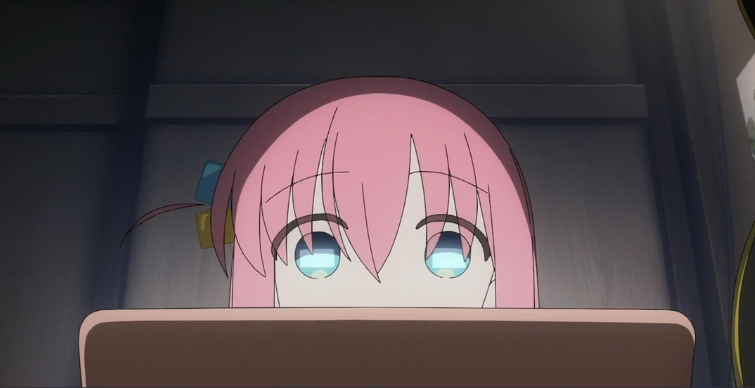
\includegraphics[width=5cm]{bocc.png}
	    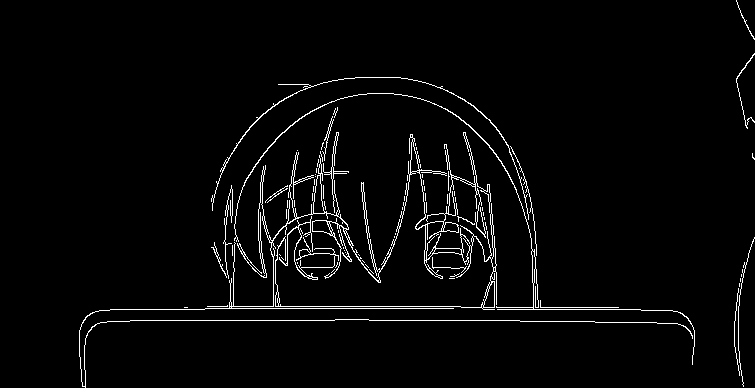
\includegraphics[width=5cm]{bocc_output_canny.png}
	    \caption{\emph{Left:} original picture, \emph{Right:} hp filtered result.}
	    \label{fig:result2}
	\end{figure}
	
	low pass filter result : 
	\begin{figure}[h!]
	    \centering
	    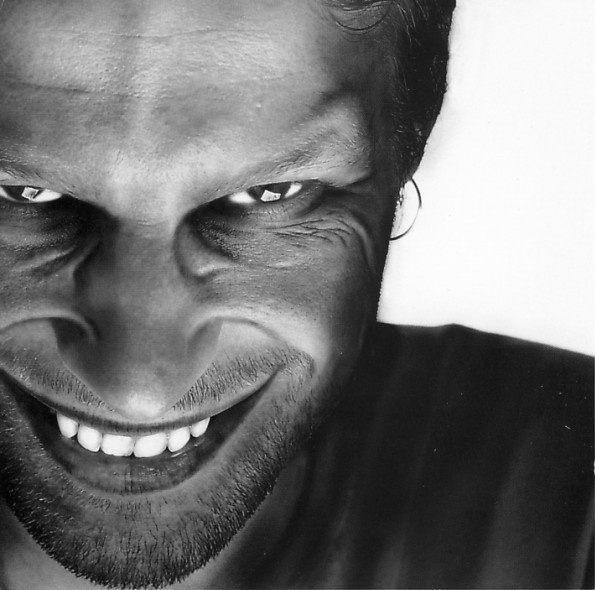
\includegraphics[width=5cm]{aphext.jpg}
	    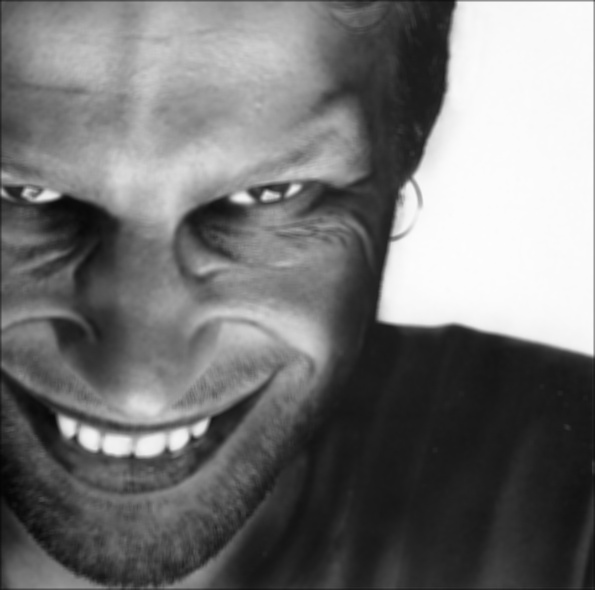
\includegraphics[width=5cm]{aphext_output_blur.jpg}
	    \caption{\emph{Left:} original picture, \emph{Right:} lp filtered result.}
	    \label{fig:result2}
	\end{figure}
	%%%%%%%%%%%%%%%%%%%%%%%%%%%%%%%%%%%
	
	% Please leave the pagebreak
	\pagebreak
	\paragraph{Q4:} How does computation time vary with filter sizes from $3\times3$ to $15\times15$ (for all odd and square sizes), and with image sizes from 0.25~MPix to 8~MPix (choose your own intervals)? Measure both using \href{https://docs.opencv.org/4.5.0/d4/d86/group__imgproc__filter.html#ga27c049795ce870216ddfb366086b5a04}{$cv2.filter2D()$} to produce a matrix of values. Use the \href{https://docs.opencv.org/4.5.3/da/d54/group__imgproc__transform.html#ga47a974309e9102f5f08231edc7e7529d}{$cv2.resize()$} function to vary the size of an image.
	Use an appropriate \href{https://jakevdp.github.io/PythonDataScienceHandbook/04.12-three-dimensional-plotting.html#Three-dimensional-Contour-Plots}{3D charting function} to plot your matrix of results, such as $plot\_surface()$ or $contour3D$.
	
	Do the results match your expectation given the number of multiply and add operations in convolution?
	See RISDance.jpg in the attached file.
	
	%%%%%%%%%%%%%%%%%%%%%%%%%%%%%%%%%%%
	\paragraph{A4:} Your answer here.

 	In order to reduce some random error, I took a measurement of average of 5 computing time.
	\begin{lstlisting}[language=Python]
import cv2
import numpy as np
import matplotlib.pyplot as plt
import time

img = cv2.imread('RISDance.jpg', 0)
m,n = img.shape
fig = plt.figure()
ax = plt.axes(projection='3d')
ker = np.array([
    [-1, 2, -1],
    [2, -4, 2],
    [-1, 2, -1]])

ker_sizes = list(range(3, 16))
scales = [0.0625, 0.125, 0.25, 0.5, 1, 2, 4, 8, 16]
X, Y  = np.meshgrid(np.log2(scales), ker_sizes)
Z = []
for r in ker_sizes:
    Z.append([])
    for s in scales:
        sum = 0
        for i in range(5):
            img_resize = cv2.resize(src=img, dsize=(0,0), fx = s, fy = s,
                                    interpolation=cv2.INTER_NEAREST)
            start_time = time.time()
            cv2.filter2D(kernel=ker, ddepth=-1, src=img_resize,
                         borderType=cv2.BORDER_DEFAULT)
            sum += time.time()-start_time
        Z[-1].append(sum/5)

ax.plot_surface(X, Y, np.array(Z), rstride=1, cstride=1,
                cmap='viridis', edgecolor='none')
plt.show()
	\end{lstlisting}

	\begin{figure}[h!]
	    \centering
	    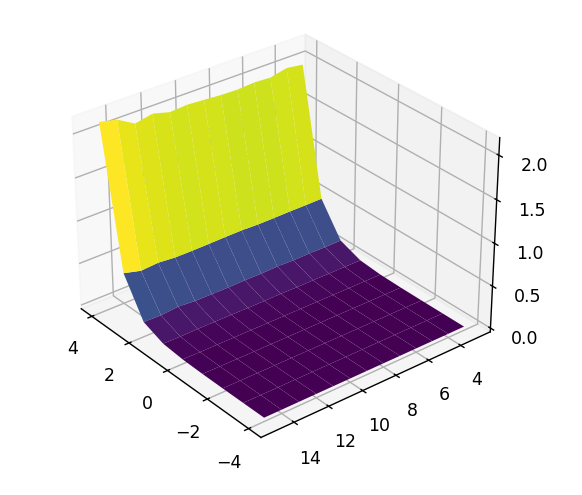
\includegraphics[width=5cm]{question4_plot.png}
	    \caption{\emph{measured computation times (filter size : 3 to 15, img scale: 0.0625x to 16x):}}
	    \label{fig:result5}
	\end{figure}
	the result clearly shows that the scale of image strongly affects the computing time, while the filter size doesn't make much sense since the image is much greater than filter.
	
	%%%%%%%%%%%%%%%%%%%%%%%%%%%%%%%%%%%
	\pagebreak
	
	% If you really need extra space, uncomment here and use extra pages after the last question.
	% Please refer here in your original answer. Thanks!
	%\pagebreak
	%\paragraph{AX.X Continued:} Your answer continued here.
	
	
	
\end{document}